% Discription of what ORB-SLAM is, how it works and implementation

\chapter{ORB-SLAM2\authorA}\label{ref:orbslam}

\section{What is ORB-SLAM?}
ORB-SLAM2 is a versatile, real-time \gls{slam} implementation which uses Mono-, Stereo- and RGB-D cameras. It's designed to generate a 3D map from prominent points in the picture and keypoints. It features loop closing, re-localization and a reusable map \cite{orbslam2}. It works in a wide variety of use cases. The \gls{slam} can be used on a small hand-held camera or drones up to self driving cars.
ORB-SLAM2 is based on ORB-SLAM and was inter alia developed by Raúl Mur-Artal who already worked on ORB-SLAM.\newline

\begin{figure}[h]
	\centering
	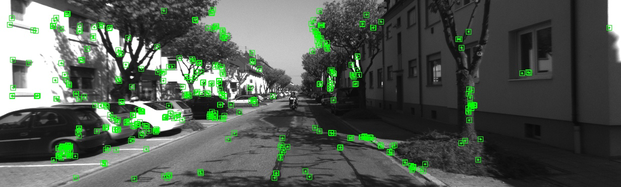
\includegraphics[width=0.8\textwidth]{./media/images/orb-slam-kitti-dataset.png}
  	\caption{ORB-SLAM Example image
  	\\Source: \url{https://tinyurl.com/ruvnj39}}
  	\label{orbslamkittidataset}
\end{figure}

\section{How does the ORB-SLAM work?}

\subsection{Extracting Keypoints}
The \gls{slam} uses a feature-based method. This means that it extracts features on prominent keypoints throughout the image input. These feature information is then distributed to all operations which handle them independent from the camera type. \cite{orbslam2} \newline\newline


This is how finding these keypoints works on different camera types:
\begin{itemize}
    \item \underline{Stereo Image} \newline
    For a stereo camera setup the keypoints get extracted for both images separately and then the left keypoints are searched on the right image. Then the found points get compared to the original ones that where found on the right side
    \item \underline{RGB-D Image} \newline
    On a RGB-D camera keypoints get extracted using prominent keypoints and then calculating the approximate position using the depth information from the information from the depth sensor.
    \item \underline{Monocular Image} \newline
    On a Monocular image the approximate position gets triangulated by using multiple images. The Disadvantage is that they don't provide a scale information and only do rotational and transnational movement estimations.
\end{itemize}

\subsection{Loop-closing and Bundle Adjustments}
Loop-closing and bundle adjustments are performed in two steps. First the loop-closing will happen when the system detects overlapping environments where the system changes scaling to reconnect certain parts as scale drifting will occur on monocular cameras.\newline
Second step is the bundle adjustment, which gets executed after a successful loop-closing, where the system tries to optimize all keypoints and keyframes using the Levenberg-Marquardt method (alternative to Gauss-Newton method).\cite{LevenbergMarquardMethod} Also the camera orientation and position will be optimized to compensate errors in tracking. All the bundle adjustment is done in a separate thread since this is a heavier task.\newline
When finished, the updated and optimized keyframes and keypoints get merged into the original keyframes and keypoints \cite{orbslam2}.

\subsection {Localization}
When a area has been mapped well in the past the \textit{Localization Mode} can be turned on which deactivates the Local Mapping and the Loop Closing thread and this saving computing power.
Locating is done by continuously comparing the previous points with the current points of the image. This works when an area is unmapped but drifting might add up.
Matching the current points with the one on the map will ensure that it is drift-free \cite{orbslam2}.

\subsection{Input/Output}
\textbf{Input Data:} rectified Monochrome/Color images\newline
\textbf{Output Data:} Rough 3D map with pixel-points and image with current prominent keypoints